% Appendix Template

\chapter{The COVID-19 Pandemic Era} \label{The COVID-19 Pandemic Era} % Change X to a consecutive letter; for referencing this appendix elsewhere, use \ref{AppendixX}


\section*{Rise of the Global Pandemic}

COVID-19 which is now officially declared as a global pandemic by the WHO was 
initially discovered in late 2019 emerging from Wuhan, People’s Republic of China.
A media statement was released by the Wuhan Municipal Health Commission confirming
multiple cases of "Viral Pneumonia from an unknown cause" on December 31$^{st}$ 2019 \cite{WMC2020}.

On January 7$^{th}$ 2020, this unknown disease was identified as the novel coronavirus by the WHO.
Three days later, the first known death caused by the coronavirus was reported \cite{WHOa2020}. The 
spread of the virus continued rapidly within China and on January 20$^{th}$ 2020, WHO reports 
the first confirmed cases outside China in Thailand, Japan, and South Korea. The very next day 
The United States reports its first confirmed coronavirus case \cite{EDW2020}. 

Following these set of events saw the introduction of quarantine protocols via lockdowns. 
Starting with Wuhan, many other cities across the world also adopted the same orders to 
suspend the spread of the coronavirus. This prompted the WHO to declare the outbreak a global public health emergency \cite{EDWa2020}. 

Within the span of a month, the death toll from COVID-19 surpassed that of SARS 
and the WHO gives the official name for the disease caused by the coronavirus "COVID-19" \cite{MCM2020}. 
The adverse effects of COVID-19 on various industries and the stock market began to 
show.

\begin{figure}[th]
\centering
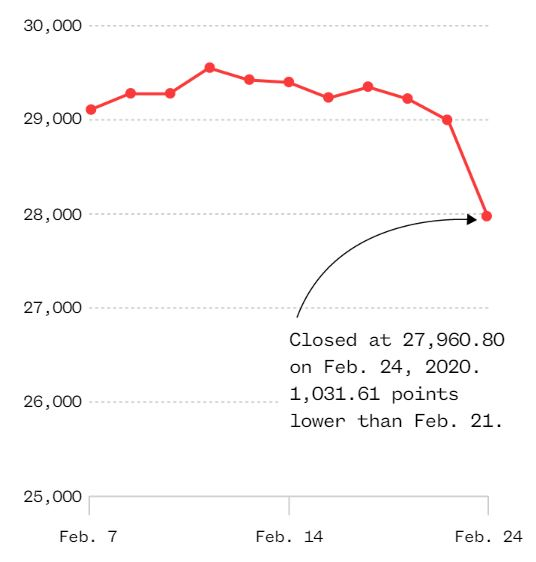
\includegraphics[height=7cm]{Images/stockMarket.JPG}
% \decoRule
\caption[Dow Jones]{Dow Jones Industrial Average experienced the worst day in two years. \cite{WBY2020}}
\label{fig:Dow Jones}
\end{figure}

Travel bans, high-profile event cancellations and activation of emergency funds were 
implemented across different countries as the number of positive cases rose above 100,000 \cite{SHA2020}.

Due to the rapid spread of the virus worldwide, on March 11$^{th}$ 2020, the WHO declares the coronavirus 
outbreak as a global pandemic \cite{JAS2020}. Over the next few months, nationwide 
lockdowns were enforced in countries such as The United Kingdom, India, South Africa, Italy, Belgium, and so on.

At the end of March 2020, The United States coronavirus cases officially surpassed China, with the former 
reporting 82,474 cases and the latter 81,961 cases.

\begin{figure}[H]
    \centering
    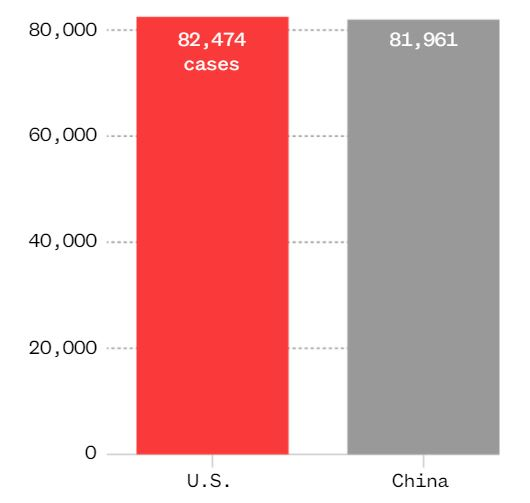
\includegraphics[height=7cm]{Images/usCases.JPG}
    % \decoRule
    \caption[COVID-19 Cases]{COVID-19 cases comparison between The United States and China \cite{GIV2020}}
    \label{fig:COVID-19 Cases Comparison}
    \end{figure}

On April 2$^{nd}$ 2020, the number of coronavirus cases worldwide surpassed 1 million with the number of deaths exceeding 51,000 \cite{PHI2020}. 
The number of positive cases doubled in April and this trend continued to follow for the next few months were as of 
October 2$^{nd}$ 2020, the total number of worldwide COVID-19 cases stand at 34,312,510, and the death toll surpassing over a million, to be precise 1,023,243 \cite{GGN2020}. 

Among the countries affected by COVID-19, The United States, India and Brazil share the 
highest percentages of positive cases.  

\begin{figure}[H]
    \centering
    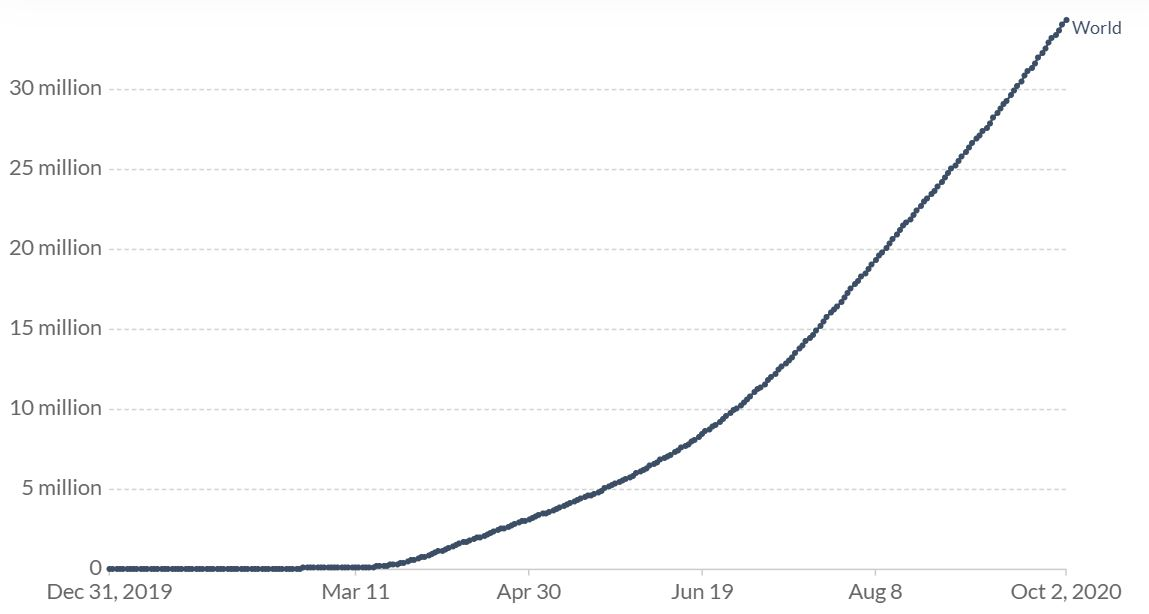
\includegraphics[width=15cm, height=6cm]{Images/totalCases.JPG}
    % \decoRule
    \caption[Total COVID-19 Cases]{Cumulative confirmed COVID-19 cases \cite{ECDC2020}}
    \label{fig:Total COVID-19 Cases}
    \end{figure}

   
\begin{figure}[H]
    \centering
    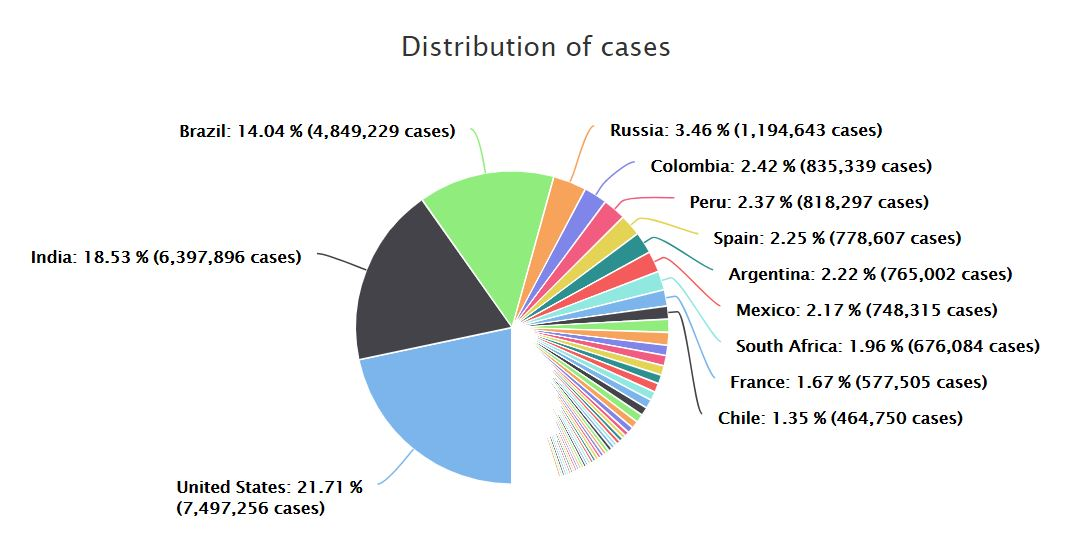
\includegraphics[width=15cm]{Images/casesDist.JPG}
    % \decoRule
    \caption[Distribution of COVID-19 Cases]{Country wise distribution of COVID-19 cases \cite{WMR2020}}
    \label{fig:COVID-19 Cases Country Wise Distribution}
    \end{figure}

    As we have now seen the major trends and events that took place in the rapid spread of COVID-19, it is upon us to work together as a community, follow the recommendations suggested by national and international healthcare agencies through which we would be able to overcome this pandemic and successfully curb the spread of the virus.